%\documentclass[]{spie}  %>>> use for US letter paper
\documentclass[12pt]{spie}
%\documentclass[a4paper]{spie}  %>>> use this instead for A4 paper
%\documentclass[nocompress]{spie}  %>>> to avoid compression of citations

\renewcommand{\baselinestretch}{1.0} % Change to 1.65 for double spacing
\usepackage{amsmath,amsfonts,amssymb}
\usepackage{graphicx}
\usepackage[colorlinks,linkcolor=blue]{hyperref}
\usepackage[colorlinks=true, allcolors=blue]{hyperref}
\usepackage{geometry}
\usepackage{url}
\usepackage[ruled, vlined, linesnumbered]{algorithm2e}
\usepackage{algorithm}
\usepackage{verbatim} 
%\usepackage[noend]{algpseudocode}
\usepackage{soul, color}
\usepackage{lmodern}
\usepackage{fancyhdr}
\usepackage[utf8]{inputenc}
\usepackage{fourier} 
\usepackage{array}
\usepackage{makecell}
\geometry{a4paper,scale=0.8}


\title{Privacy-Preserving AI for COVID-19 CT Diagnosis: with Design of an Interactive Web-Based Toolkit}
\author[a] {Hansheng GUO}
\author[b] {Zhiyuan YU}
\author[c] {Jiuming WANG}
\affil[d]{The Chinese University of Hong Kong\\

Sha Tin, N.T, Hong Kong S.A.R., China\\} 

\authorinfo{Further author information: (Correspondence to GUO Hansheng)\\GUO Hansheng: E-mail: hsguo@link.cuhk.edu.hk}

% Option to view page numbers
\pagestyle{empty} % change to \pagestyle{plain} for page numbers   
\setcounter{page}{-1} % Set start page numbering at e.g. 301

\begin{document} 

\maketitle

\begin{abstract}
Privacy protection is of vital importance when artificial intelligence is applied to data associated with sensitive or private information, such as personal medical history. Therefore, effective privacy-preserving AI algorithms could gain more trust from doctors and patients, hence increasing their popularity in practice. In the most recent two years, as the ongoing COVID-19 pandemic keeps posing constant threats to the world, more and more efforts have been made to help medical professionals make an efficient and accurate diagnosis for clinically infection-suspicious patients. One commonly used method is to examine the CT scans of the patients for abnormalities. This project introduces a web-based toolkit by implementing the federated learning technique to facilitate the diagnosis of COVID-19. By adopting the federated learning approach, the model is able to bring together the data across the world to train itself while preserving personal information. The application of this toolkit is not limited to facilitating the diagnosis; it could also benefit the training of students from medical schools or junior professionals in the hospital.  
\end{abstract}

% Include a list of keywords after the abstract 
\keywords{COVID-19, deep learning, federated learning, privacy protection, image segmentation, AI-facilitated diagnosis}

\newpage

\tableofcontents

\newpage

\section{Introduction}
Since the outbreak of coronavirus (COVID-19 or SARS-CoV-2), the entire world has been fighting against it in multiple domains including public healthcare, the economy, and even personal entertainment[2]. Although the public vaccination scheme is gradually proceeding in many regions of the world, the finding of new mutant viruses keeps posing new threats to us. Furthermore, less-developed regions with insufficient medical resources lack professional and qualified radiologists and doctors to conduct an accurate and efficient diagnosis. Without an effective diagnosis being made, severe complications of the infection of COVID-19 would be displayed by the patient. Therefore, it is of vital importance for the healthcare community to be able to share the diagnosis information and valuable cases to identify the common symptoms among patients infected with COVID-19. 


COVID-19 belongs to a type of contagious virus that could cause mild to severe symptoms from fatigue to respiratory system failure and other common symptoms shared with pneumonia[4]. For patients who are highly suspicious of infection with COVID-19, the CT scanning result could be helpful in facilitating the diagnosis. In the CT scans from confirmed cases, ground-glass opacities could be observed in the early stage and consolidation might also occur as the condition worsens for the patient. The following images show how a COVID-19-infected CT scan progresses as the disease gradually becomes severer.
\begin{figure}[H]
  \centering
  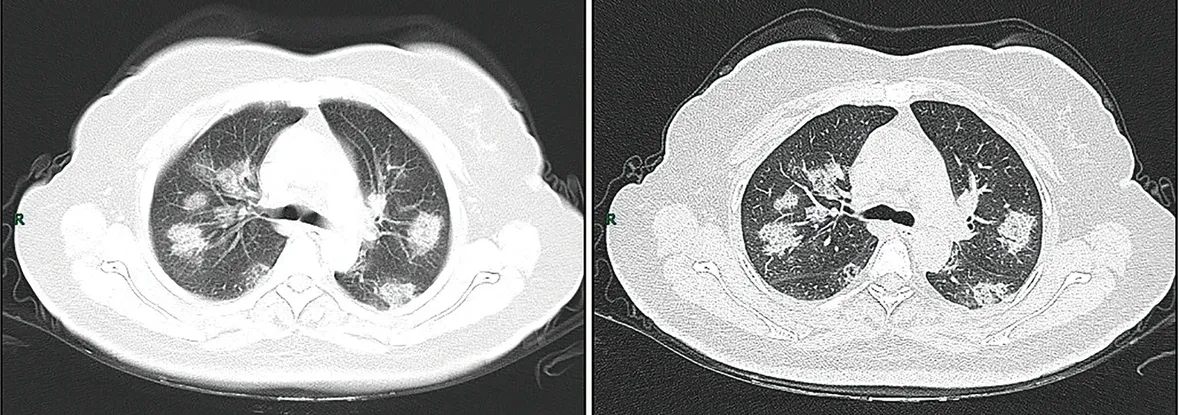
\includegraphics[width=0.7\textwidth]{scan.png} 
   \caption{CT scan of COVID-19 infected lungs in different 
   stages [1]}
   
\end{figure}

\section{Theory}
\subsection{Semantic Image Segmentation}
The goal of semantic segmentation is to classify each pixel into one of the pre-set classes. It's now one of the most famous tasks in computer vision based on deep learning. The task can help machines better understand the image scene and show the global context of the image. It's now widely used in several industries including security, self-driving car, and also medical diagnosis[5].

\subsection{Federated Learning}
Privacy is of great significance especially when Artificial Intelligence is applied to healthcare topics. In this project, we adopted a technique, namely federated learning, to address the potential risk of leaking personal private health information to third parties. This section introduces the essential knowledge about federated learning and how it is applied in our model.

Theoretically, when there are multiple data sources $F_{i}$ involved in one training task, all the data $D_{i}$ from these sources will be merged as one training dataset $D$ to train the model[6]. However, due to various reasons such as legislation and privacy protection, such an approach to gathering data across institutions and laboratories is oftentimes not practical in reality, especially when it comes to healthcare applications. Therefore, in order to resolve this problem, we applied the federated learning method. Federated learning is defined as the training method by which each single separated data source $F_{i}$ is not necessarily required to submit its data $D_{i}$ to the coordinator, and the model could be trained separately on each $D_{i}$ without being merged together. By considering the different characteristics of the data acquired, we could divide the federated learning approach into three different categories, namely horizontal, vertical federated learning, and federated transfer learning. Those learning techniques differ in terms of the overlapping of data between different data sources. For instance, if multiple data sources include the same feature, then it is referred to as “horizontal”; if the same user contributed to multiple data sources, then the technique is called "vertical". In our project, we specifically adopted horizontal federated learning where multiple data sources all provide us with the CT scan images taken from COVID-19 infected cases[7]. 
\begin{algorithm}
\DontPrintSemicolon
\SetKwProg{Fn}{Function}{ is}{end}
\Fn{train\_model()} {
  \ForEach{$D_{ii}$: $D_{i}$} {
    model\_train\_on($D_{ii}$, $param_{i}$) \;
  }
  \Return{$param_{i}$}
}
\BlankLine
\SetKwProg{Fn}{Function}{ is}{end}
\Fn{coordinate(i: federate training result $F_{i}$, params, key)} {
  \ForEach{federation $F_{i}$}{
    send the params to $F_{i}$ via key;
  }
}
\BlankLine
\SetKwProg{Fn}{Function}{ is}{end}
\Fn{main(i: $F_{i}$, $D_{i}$, key)} {
  \ForEach{federation $F_{i}$} {
    send the encryption key to $F_{i}$;
  }
  params = [];\\
  \While{model performance < expectation}{
    \ForEach{federation $F_{i}$}{
    param = train\_model($D_{i}$);\\
    params.append(param);
  }
  coordinate($F$, params, key);
  }
}
\label{algo:1}
\caption{Federated Learning Algorithm Framework}
\end{algorithm}
First, he coordinator $C$ sends the encryption key to the data sources $F_{i}$ Isolated data sources $F_{i}$ and $F_{j}$ trained the mode on their data $D_{i}$ and $D_{j}$ respectively.
After that, $F_{i}$ and $F_{j}$ communicate with each other regarding the gradient updates and other training-related information with each other by using the encryption key sent by the coordinator.
Loss and other information are computed separately and then sent to the coordinator $C$ using the encryption key.
Then the coordinator $C$ receives the training updates from different sources $F_{i}$ and computes the overall parameter update.
Eventually, the overall updates are distributed to the data sources for updating their parameters.
This procedure is repeated until the overall model converges or reaches a satisfying performance. A pseudo-code illustration of the federated learning framework is depicted above.

\section{Method}
\subsection{Transfer Learning}
The effect of the deep learning model is extremely dependent on data, we use transfer learning to improve the effect. The dataset includes 32,120 axial CT slices (from body parts of the liver, lung, mediastinum, kidney, pelvis, bone, abdomen, and soft tissue) from 10,594 studies from 4427 unique patients, which is the most comprehensive open-source data for CT lesions currently[10]. 

For the network architecture of our model, we used an improved version of ResNet18, which is a medical domain-customized 2D CNN network for object detection on the original RetinaNet backbone. We combined three adjacent CT axial slices as the model input. Our model was firstly pretrained on the DeepLesion dataset and then we fine-tuned it with internal COVID-19 training images[8].

\subsection{Federated Learning}
In order to protect data privacy during model training, the team of our adopted model studied the feasibility of federated learning in three local hospitals, where each center represents a node[3]. There is no need to share data across sites, and the model benefits from the generalization achieved by multi-center learning, including different data sources. This decentralized scheme trains a single model on the local node and exchanges it to network parameters to update the global model stored on the central server at a specific frequency. In each iteration of the joint update, the central server first aggregates all local models and uses them to update the global model parameters using the joint averaging algorithm. The updated global model is generated by using the weighted average of the parameters from all local models, weighted in proportion to the sample size on each node, and provided by the local node to the global server. Next, the central server distributes the updated global model to the local nodes, and then each node continues to perform local optimization based on the updated global model.

\section{Result}

\begin{figure}[H]
  \centering
  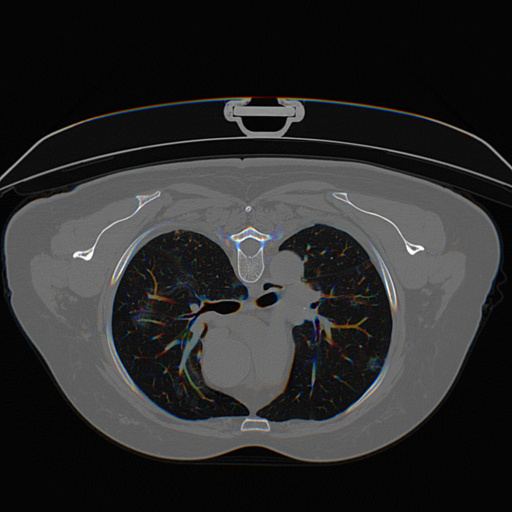
\includegraphics[width=0.3\textwidth]{ct01-1.png} 
   \caption{Test Picture 1}
\end{figure}
\begin{figure}[H]
  \centering
  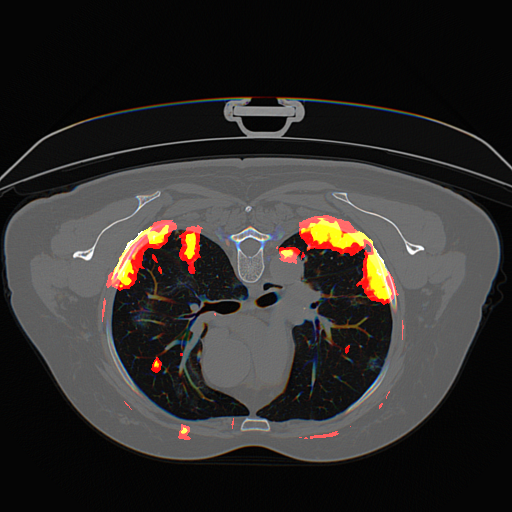
\includegraphics[width=0.3\textwidth]{P1-1.png} 
   \caption{Test Result 1}
\end{figure}

\begin{figure}[H]
  \centering
  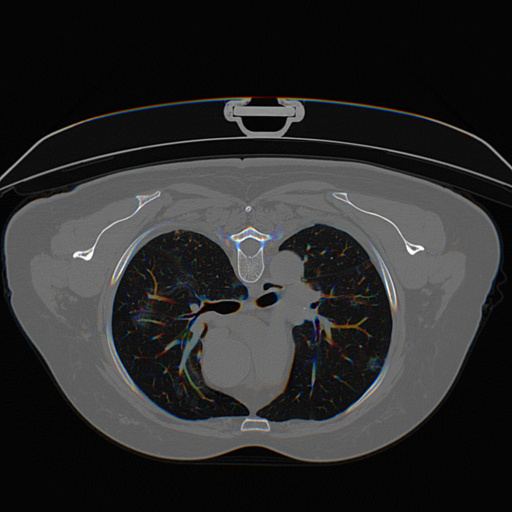
\includegraphics[width=0.3\textwidth]{ct01-2.png} 
   \caption{Test Picture 2}
\end{figure}
\begin{figure}[H]
  \centering
  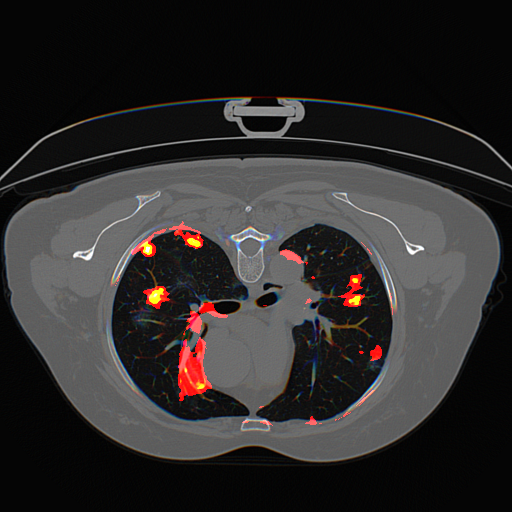
\includegraphics[width=0.3\textwidth]{P1-2.png} 
   \caption{Test Result 2}
\end{figure}

\begin{figure}[H]
  \centering
  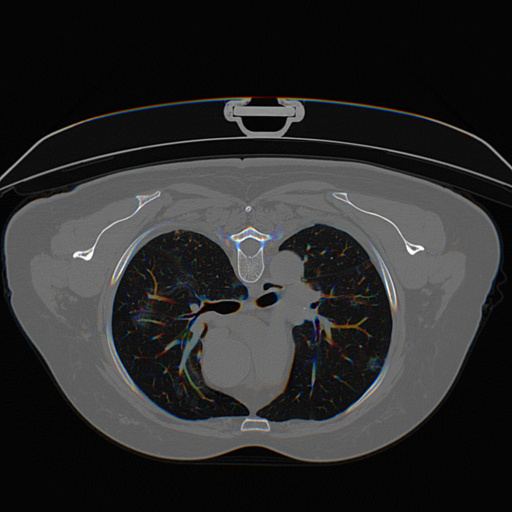
\includegraphics[width=0.3\textwidth]{ct01-3.png} 
   \caption{Test Picture 3}
\end{figure}
\begin{figure}[H]
  \centering
  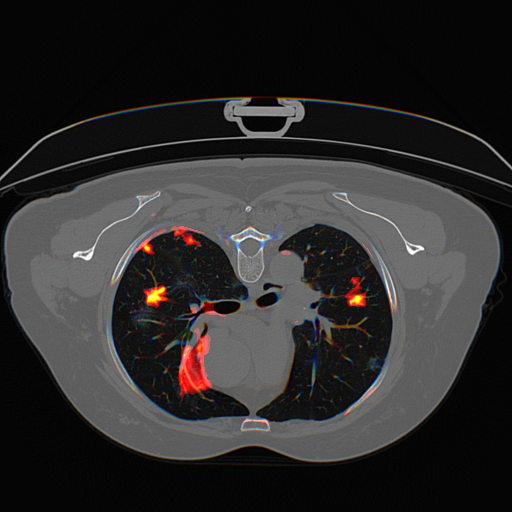
\includegraphics[width=0.3\textwidth]{P1-3.png} 
   \caption{Test Result 3}
\end{figure}

\section{Application}
Based on our high accuracy and privacy-preserving model, we developed the following applications to put it into use.
\subsection{Helper for Medical Diagnosis}
In many economically underdeveloped areas, the level of doctors is limited and the epidemic is often the most severe. Our model can quickly show the areas that may be infected by the virus and provide doctors with reference. Even a novice doctor can make a fast and accurate medical diagnosis with our tool.
\subsection{Condition Tracker}
In addition to the detection and segmentation of abnormal areas, our model can also give the area and volume percentage of the infected part. Only need to provide multiple CT images within a few days, the model can quantify the patient's physical recovery so that it can help doctors judge whether the treatment is effective and the patient's recovery speed.
\subsection{Educational Toolkit}
It is also a perfect tool to educate medical students. The model randomly gives a CT picture, the user needs to enter whether the patient is infected, the proportion of the infected area and mark the area. Then the software will automatically judge the correctness of the answer and help students correct and improve. We are building a web game for this application now.
\newpage
% References
\section{references}
$\left[1\right]$ Military Medical Research volume 7, Article number: 4 (2020)\\
$\left[2\right]$ COVID C. Global cases by the Center for Systems Science and Engineering (CSSE) at Johns Hopkins University (JHU). ArcGIS. Johns Hopkins CSSE (2021).\\
$\left[3\right]$ Dou, Q., So, T.Y., Jiang, M. et al. Federated deep learning for detecting COVID-19 lung abnormalities in CT: a privacy-preserving multinational validation study. npj Digit. Med. 4, 60 (2021). https://doi.org/10.1038/s41746-021-00431-6\\
$\left[4\right]$ Long, C., Xu, H., Shen, Q., Zhang, X., Fan, B., Wang, C., & Li, H. (2020). Diagnosis of the Coronavirus disease (COVID-19): rRT-PCR or CT?. European journal of radiology, 126, 108961.\\
$\left[5\right]$ Minaee, S., Boykov, Y. Y., Porikli, F., Plaza, A. J., Kehtarnavaz, N., & Terzopoulos, D. (2021). Image segmentation using deep learning: A survey. IEEE Transactions on Pattern Analysis and Machine Intelligence.\\
$\left[6\right]$ Konečný, J., McMahan, H. B., Yu, F. X., Richtárik, P., Suresh, A. T., & Bacon, D. (2016). Federated learning: Strategies for improving communication efficiency. arXiv preprint arXiv:1610.05492.\\
$\left[7\right]$ Li, W., Milletarì, F., Xu, D., Rieke, N., Hancox, J., Zhu, W., ... & Feng, A. (2019, October). Privacy-preserving federated brain tumour segmentation. In International workshop on machine learning in medical imaging (pp. 133-141). Springer, Cham.\\
$\left[8\right]$ Khan, S., Islam, N., Jan, Z., Din, I. U., & Rodrigues, J. J. C. (2019). A novel deep learning based framework for the detection and classification of breast cancer using transfer learning. Pattern Recognition Letters, 125, 1-6.\\
$\left[9\right]$ Kaissis, G. A., Makowski, M. R., Rückert, D. & Braren, R. F. Secure, privacy-preserving and
federated machine learning in medical imaging. Nat. Mach. Intell. 2, 305–311 (2020)\\
$\left[10\right]$ Yan, K., Wang, X., Lu, L. & Summers, R. M. DeepLesion: automated mining of largescale lesion annotations and universal lesion detection with deep learning. J.
Med. Imaging 5, 036501 (2018).
\\
\\
\textbf{Video Download Link: } \href{https://www.dropbox.com/s/qrhwq4ypqo152ij/Emedic-video.mp4?dl=0}{Click here} 
\end{document} 
